% swrMOL.tex
% Source: "SWR and the meaning of life" by Jim Tregellas VK5JST,
%   Amateur Radio (WIA) Vol. 89 No. 2, 2021. (Originally WIA_MEMBER_ARMAG_2021_2_Mar_Apr.PDF)
% Converted from PDF to LaTeX on 2026-10-30.
%
% Notes on figures:
%   * Figure 1 and Figure 2 in the original are data TABLES (not raster images).
%     They are reconstructed here as LaTeX tabulars: Figure 1 uses the IARU
%     S-meter standard (S9 = 50 uV into 50 ohm, 6 dB / S-point); Figure 2 uses
%     the reflected-power formula loss% = 100 * ((SWR-1)/(SWR+1))^2.
%   * Figure 3 is a vector plot in the PDF. It is redrawn here with pgfplots from
%     the standing-wave voltage formula V(x) = sqrt(1 - 2*Gamma*cos(4*pi*x) + Gamma^2),
%     with Gamma = (SWR-1)/(SWR+1), x in wavelengths [0,1].
%   * The 144 MHz beacon map is the only true raster image; it is embedded from
%     images/swrMOL_beacon.jpg (extracted from the PDF).
%
% Compile with: pdflatex swrMOL.tex   (or xelatex)

\documentclass[11pt]{article}

\usepackage[utf8]{inputenc}
\usepackage{graphicx}
\usepackage{booktabs}
\usepackage{url}
\usepackage{caption}
\usepackage{geometry}
\usepackage{pgfplots}
\geometry{margin=1in, headheight=0pt}
\pgfplotsset{compat=1.18}

\title{SWR and the meaning of life}
\author{Jim Tregellas VK5JST}
\date{Amateur Radio (WIA) Vol.\ 89 No.\ 2, 2021}

\begin{document}
\maketitle

\section*{SWR and the meaning of life}

We all know about SWR -- standing wave ratio -- because, over our lives we have
all gathered a lot of information on the subject from our ham and CB friends, and
other reliable sources, such as the American educational movie series entitled
``Smokey and the Bandit''. 

All of these sources clearly demonstrate that unless
the ``SWR'' of our antenna system is less than 1.05, then we will not be heard,
our finals will blow up, we will get RF burns from the metal parts of our
microphones and rigs, and we may actually end up sterile from the excessive RF in
the shack. Right? Errm, well, not quite.

Amateur radio is full of tall tales and true, and nothing has more nonsense
spoken about it than the SWR of antenna systems. So, let's look at some hard
facts and try to establish some truth.

\subsection*{About signal strength}

Back in the 1930s, it was generally agreed that 50 microvolts RMS of RF at the
input terminals of a radio was an S9 signal (large), but that was about the
extent of the agreement because receiver input impedances varied widely and so
did the receiver automatic gain control (AGC) characteristics, noise performance
and overall gain. 

It was not until the early 1980s that an attempt at some
standardization was made by the International Amateur Radio Union (IARU) and
signal levels were defined that should produce particular readings on a
receiver's S-meter. The receiver input impedance assumed for these ``standards''
was 50 ohms and the voltage levels defined are shown in Figure 1.

Note that a change of one S-point doubles or halves the voltage to be found at
the receiver input (or a 6 dB change). This logarithmic scale has some
interesting consequences. Say a distant transmitter of 100 Watts is producing a
strength seven (S7) level in your receiver. To boost the received signal to S8,
the voltage at the receiver input must double, and so the transmitter power must
be quadrupled to 400 Watts to cause this. An S9 signal level will require a
transmitter power of 1600 Watts!

Also note that this quadrupling of transmitter power produces a fairly minor
change in the received audio level due to the receiver's AGC action. It is worth
noting that, even in these days of very advanced receivers, AGC action is seldom
exactly logarithmic and S-meters still typically tell the small lies loved by
salespeople everywhere as they boast about the behavior of their products.

\begin{figure}[htbp]
  \centering
  \begin{tabular}{cc}
    \toprule
    S reading   & Input signal ($\mu$V) \\
    \midrule
    S1          & 0.2   \\
    S2          & 0.4   \\
    S3          & 0.8   \\
    S4          & 1.6   \\
    S5          & 3.2   \\
    S6          & 6.3   \\
    S7          & 12.5  \\
    S8          & 25.0  \\
    S9          & 50.0  \\
    S9 + 10 dB  & 160.0 \\
    S9 + 20 dB  & 500.0 \\
    \bottomrule
  \end{tabular}
  \caption{Figure 1. Signal strengths and the related receiver input voltages
    (IARU 50-ohm S-meter standard: S9 = 50~$\mu$V, 6~dB per S-point).}
  \label{fig:fig1}
\end{figure}

\subsection*{Power loss at various SWR levels}

The next item that must be addressed is what power loss is implied by various
SWR figures? 

Have a look at Figure 2 and prepare to be surprised. Even at an SWR
of 3.0, the power loss in the antenna system is just 25~\%, which, given the
four-fold increase in power level needed to move just one S-point, only
represents a change of a very small part of an S-point, and essentially no change
in the received audio level at all. 

For an SWR of 1.5 or less (4~\% loss), you
will not even see the S-meter needle move, and you will certainly not be able to
detect any change at all in receiver audio level. 

So given the above, why all
the fuss about SWR?

\begin{figure}[htbp]
  \centering
  \begin{tabular}{cc}
    \toprule
    SWR   & Power loss (\%) \\
    \midrule
    1.0   & 0.0   \\
    1.1   & 0.2   \\
    1.2   & 0.8   \\
    1.3   & 1.7   \\
    1.4   & 2.8   \\
    1.5   & 4.0   \\
    1.75  & 7.4   \\
    2.0   & 11.1  \\
    2.5   & 18.4  \\
    3.0   & 25.0  \\
    5.0   & 44.4  \\
    10.0  & 66.9  \\
    \bottomrule
  \end{tabular}
  \caption{Figure 2. The power lost (reflected) at various levels of SWR,
    computed as $100\times((SWR-1)/(SWR+1))^2$.}
  \label{fig:fig2}
\end{figure}

\subsection*{Standing waves in an antenna system}

Standing waves develop in an antenna system as a result of the impedance of the
system not matching the output impedance of the transmitter. As the output of
the transmitter moves through a series of cycles of a (hopefully) good clean
sine wave, each cycle moves down the transmission line toward the antenna and
away from the transmitter at either the speed of light (open-wire lines) or some
fraction of the light speed. 

In the case of coaxial cables with solid plastic
dielectrics such as RG58, these wave fronts move at around 66~\% of the velocity
of light (or RF). Cables with foam dielectrics have lower losses and faster
moving wave fronts (typically 0.8--0.9 of light's velocity). The speed of
propagation relative to the speed of light is known as the ``velocity factor''.

When each wave front reaches the system termination, its energy may be totally
absorbed and radiated by the antenna (a perfect match of 50 ohms), or some
energy may be reflected back towards the transmitter. 

In the first case, as
there is no reflected energy, no standing wave can develop and the RF voltage
along the transmission line will be exactly the same at all points on the line.
This is illustrated in Figure 3 by the yellow trace in the graph.

In the second case, the amount of reflected energy will be determined by how
close the terminating impedance is to 50 ohms. For a SWR of 1.5 (little
reflected energy) the terminating resistor in a 50 ohm system can be either 75
ohms or 33.33 ohms as both of these generate this SWR figure. 

This same idea of
two different loads generating the same SWR also applies to a system with either
a shorted or open-circuit load. No energy can be absorbed in these loads and so
the SWR is infinity (the yellow trace).

In Figure 3, note that, as the load SWR moves away from the perfect 1.0 in
either direction (either greater or lesser impedances than the perfect 50 ohm
termination), the voltage maximums and minimums along the transmission line
increase as the forward and back waves interact. And this is what causes the
concern with SWR figures.

It is also worth reflecting on what happens to the RF current along such a
transmission line. It has the opposite shape to the standing wave for voltage.
As power is being transmitted, when the voltage is maximum then the current is
minimum, and vice versa. 

The final part of the picture is that transmission
lines are seldom of the right length. It is entirely possible that the
transmitter output might just be coupled to a line with a voltage or current
maximum that appears right at the transmitter output and so places the output
devices under the maximum possible stress.

\begin{figure}[htbp]
  \centering
  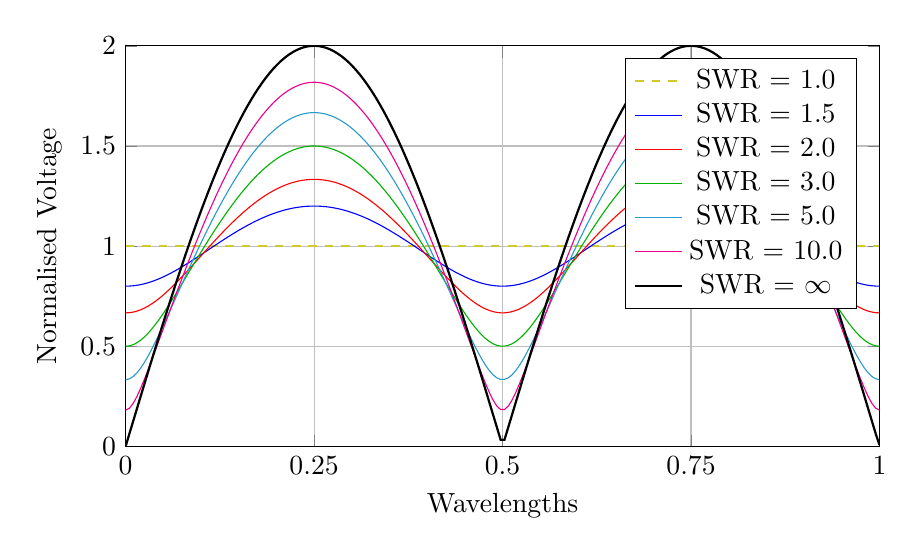
\begin{tikzpicture}
    \begin{axis}[
      width=0.92\textwidth, height=0.55\textwidth,
      xlabel={Wavelengths},
      ylabel={Normalised Voltage},
      xmin=0, xmax=1, ymin=0, ymax=2,
      xtick={0,0.25,0.5,0.75,1},
      ytick={0,0.5,1,1.5,2},
      grid=major,
      legend pos=north east,
      samples=200,
      domain=0:1,
    ]
      % SWR = 1.0 : flat line (yellow trace in original)
      \addplot[domain=0:1, yellow!80!black, thick, dashed] {1};
      \addlegendentry{SWR = 1.0}
      % SWR = 1.5 : Gamma = 0.2
      \addplot[domain=0:1, blue] {sqrt(1 - 0.4*cos(deg(4*pi*x)) + 0.04)};
      \addlegendentry{SWR = 1.5}
      % SWR = 2.0 : Gamma = 1/3
      \addplot[domain=0:1, red] {sqrt(1 - 0.6667*cos(deg(4*pi*x)) + 0.1111)};
      \addlegendentry{SWR = 2.0}
      % SWR = 3.0 : Gamma = 0.5
      \addplot[domain=0:1, green!70!black] {sqrt(1 - 1.0*cos(deg(4*pi*x)) + 0.25)};
      \addlegendentry{SWR = 3.0}
      % SWR = 5.0 : Gamma = 2/3
      \addplot[domain=0:1, cyan!80!black] {sqrt(1 - 1.3333*cos(deg(4*pi*x)) + 0.4444)};
      \addlegendentry{SWR = 5.0}
      % SWR = 10.0 : Gamma = 9/11
      \addplot[domain=0:1, magenta] {sqrt(1 - 1.6364*cos(deg(4*pi*x)) + 0.6694)};
      \addlegendentry{SWR = 10.0}
      % SWR = infinity : Gamma = 1
      \addplot[domain=0:1, black, thick] {sqrt(2 - 2*cos(deg(4*pi*x)))};
      \addlegendentry{SWR = $\infty$}
    \end{axis}
  \end{tikzpicture}
  \caption{Figure 3. Illustrating the voltage maximums and minimums
    (``maxima and minima'') along a transmission line at differing SWR values.
    Curves are the normalised standing-wave voltage
    $V(x)=\sqrt{1-2\Gamma\cos(4\pi x)+\Gamma^2}$ with
    $\Gamma=(SWR-1)/(SWR+1)$, $x$ in wavelengths.}
  \label{fig:fig3}
\end{figure}

\subsection*{A design compromise}

So it is worth looking at Figure 3 in more detail, because it clearly shows the
compromise a design engineer must make when designing an RF output stage. On one
side is a sales engineer screaming that, to compete with the opposition, he
needs the maximum possible output power and on the other side is an accountant
moaning about the costs of expensive RF output devices. 

The nett result of all
this pressure is that the RF output devices in a transceiver are generally
flogged to within an inch (cm~\dots) of their lives, and little safety margin is
left. Typical industry practice is therefore to provide full output power up to
an SWR of 1.5 (25~\% over-voltage) and after this, to back-off the drive to the
RF output stages with ALC. And this protection happens fast. If you happen to
have an antenna system with an SWR of 3.0 then you will be lucky if your modern
100 Watt transmitter is actually putting out 20 Watts.

Of course, a lot of the mythology about SWR stems from the early days of CB,
when output stages were totally unprotected (costs again), and even the shortest
exposure of a transceiver output stage to an open or shorted line would result
in either 200~\% overvoltage or current that would immediately destroy the
output transistors. 

It should also be pointed out that the tube output stages of
old ``boat anchor'' rigs are way less likely to be damaged by these factors.
First, these output stages almost always have ``Tune'' and ``Load'' controls
that allow impedances other than 50 ohms to be perfectly matched and, secondly,
tubes have far greater margins available to deal with overloads anyway. 

Most
``boat anchors'' will happily deal with SWRs of 3.0 or more without complaint.

Finally, it is interesting that many international broadcasting stations that
have to be very frequency agile above the 40m ham band to take advantage of
current propagation conditions use antenna systems with SWR figures of up to
9.0. Why? Because it is cheaper to design a very tolerant transmitter output
stage than to design and construct a very wideband antenna system.

\subsection*{Summarising}

So in summary, provided your SWR is less than 1.5, there will be no ill effects
at all -- and with most boat anchors you can get away with murder. But, if you
want to be heard all of the preceding discussion assumes that you have an
efficient antenna system. You can easily get a very low SWR at 2m by connecting
a 144 MHz transceiver to a 100 metre length of RG58 with the far end being open
circuit. Lots of hot plastic, no reflected power back to the transceiver, and a
measured SWR of less than 1.1:1!

\section*{144 MHz beacon in South Atlantic heard 7000 km away in France}

The recently installed 144 MHz beacon on St Helena Island in the South Atlantic
off the coast of West Africa, was copied by Jeff FY0F on 5 March 2021. As
reported by John EI7GL, the path is almost 7000 km, as illustrated on the map
here. 

FY0F recorded signals of the ZD7GWM beacon on 144.475 MHz for a period
just shy of two hours, from around 9pm to 11pm local time. This time period,
together with the signal characteristics, strongly suggests the propagation was
Class 2 (evening-type) transequatorial propagation (TEP). Check out this
29-second recording: \url{https://soundcloud.com/f0fyf/beacon2}

To copy the beacon, Jeff was using a stack of 2~$\times$~9-element Yagis at 7m
height above ground, mounted on a temporary mast. 

There is some discussion
online about the audio recordings of ZD7GWM off-air by FY0F during this session,
which don't match some characteristics of other recordings of the beacon. 

To
learn more about Evening Type Transequatorial VHF Propagation, visit:
\url{http://home.iprimus.com.au/toddemslie/eTEP-Harrison.htm}

Roger Harrison VK2ZRH

\begin{figure}[htbp]
  \centering
  \includegraphics[width=0.6\textwidth]{images/swrMOL_beacon.jpg}
  \caption*{Reception of the St Helena beacon ZD7GWM on 144 MHz by FY0F in
    France, March 2021 -- approximately 7000 km (great-circle path shown).}
  \label{fig:beacon}
\end{figure}

\end{document}
